\documentclass[12pt]{article}
\bibliographystyle{ieeetr}
\usepackage[a4paper, total={6in, 8in}]{geometry}
\usepackage{amsmath}
\usepackage[colorlinks=false]{hyperref}
\usepackage{blindtext}
\usepackage{graphicx} % Required for inserting images
\usepackage[english]{babel}
\usepackage{pdfpages}
\usepackage{xargs}                      % Use more than one optional parameter in a new commands
%\usepackage[pdftex,dvipsnames]{xcolor}  % Coloured text etc.
%
\usepackage[colorinlistoftodos,prependcaption,textsize=tiny]{todonotes}
\newcommandx{\unsure}[2][1=]{\todo[linecolor=red,backgroundcolor=red!25,bordercolor=red,#1]{#2}}
\newcommandx{\change}[2][1=]{\todo[linecolor=blue,backgroundcolor=blue!25,bordercolor=blue,#1]{#2}}
\newcommandx{\info}[2][1=]{\todo[linecolor=OliveGreen,backgroundcolor=OliveGreen!25,bordercolor=OliveGreen,#1]{#2}}
\newcommandx{\improvement}[2][1=]{\todo[linecolor=Plum,backgroundcolor=Plum!25,bordercolor=Plum,#1]{#2}}
\newcommandx{\thiswillnotshow}[2][1=]{\todo[disable,#1]{#2}}

\title{GreenBlocks - SMT PdM}
\author{mbelanger.poly}
\date{August 2023}


\begin{document}

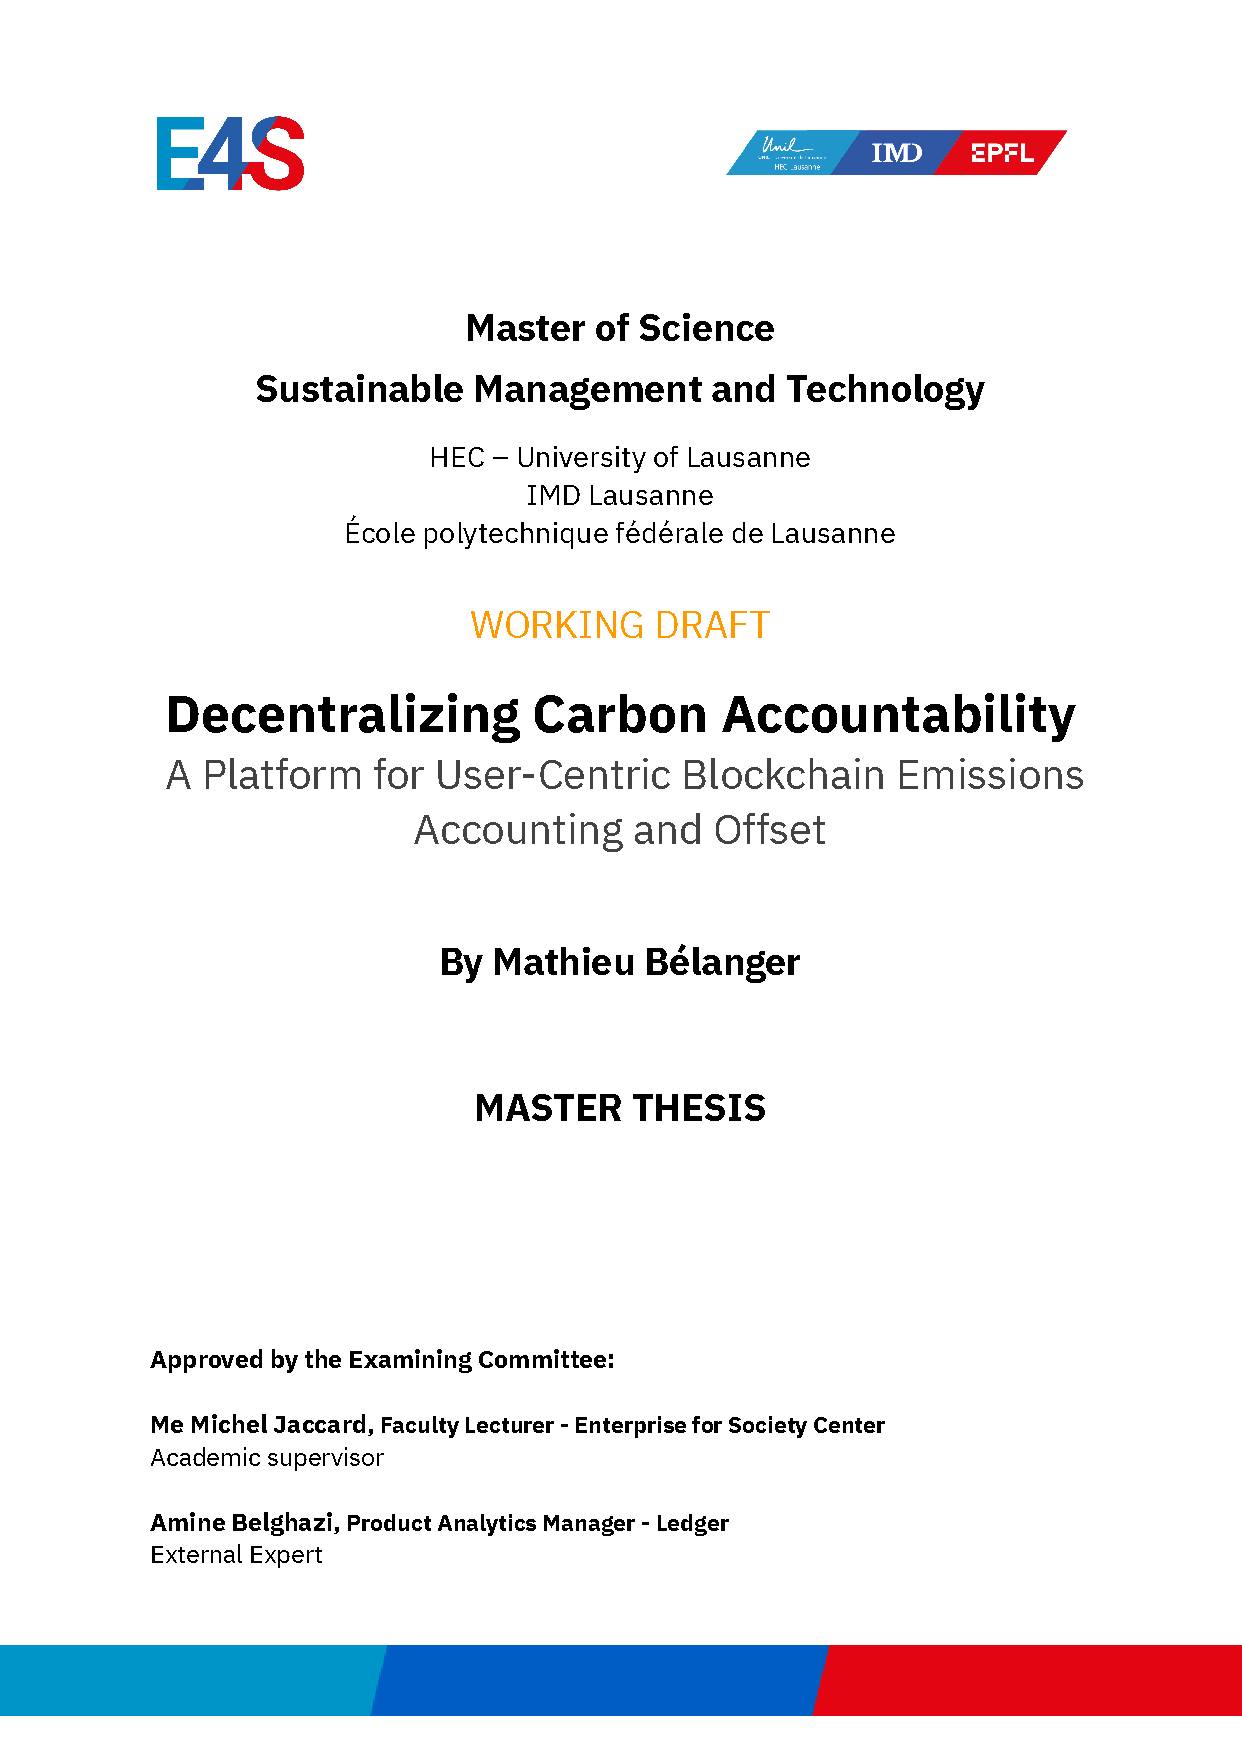
\includepdf[pages={1-2}]{cover.pdf}

\tableofcontents

\section{Introduction}
\blindtext
\cite{nakamoto_bitcoin_2008}
\cite{aysan_blockchain-based_2021}
\cite{de_vries_revisiting_2022}




\subsection{Background and Motivation}
\blindtext
\subsection{Problem Statement}
\subsection{Research Questions and Ojbectives}
\subsection{Scope and Limitations}
\subsection{Structure of the Thesis}


\section{Litterature Review}
\subsection{Evolution of Blockchain Technology}
\subsection{Environmental Impact of Blockchains}
\subsubsection{Energy Consumption and Related Emissions}
\subsubsection{Current Measurement Methodologies and Datasets}
\subsection{User-Level Emissions Attribution}


\section{Methodology}
\subsection{Overview of the attribution strategy}
\subsection{User-Level Emission Atrribution Model}
\subsubsection{Historical Blockchain Emissions Data}
\subsubsection{User attribution}
\subsubsection{Responsibility share}
\subsubsection{Weighting factors}
\subsubsection{Cumulative Emissions}
\subsection{Data Sources and Collection}


\subsubsection*{General Form}
\begin{equation}
\text{Footprint}_{chain}(t) = \int_{0}^{t} \left[ \text{EmissionRate}_{chain}(\tau) \cdot \left( \alpha_{chain} \text{BalanceShare}(\tau) + \gamma_{chain} \text{Transactions}(\tau) \right) \right] d\tau
\end{equation}




\subsubsection*{Value-Transfer Chains (VTC)}
\begin{equation}
\text{Footprint}_{VTC}(t) = \int_{0}^{t} \left[ \text{EmissionRate}_{VTC}(\tau) \cdot \left( \alpha_{VTC_i} \text{BalanceShare}(\tau) + \gamma_{VTC_i} \text{Transactions}(\tau) \right) \right] d\tau
\end{equation}

\subsubsection*{General Purpose Chains (GPC)}
\begin{equation}
\text{Footprint}_{GPC}(t) = \int_{0}^{t} \left[ \text{EmissionRate}_{GPC_j}(\tau) \cdot \left( \alpha_{GPC_j} \text{BalanceShare}(\tau) + \beta_{GPC_j} \text{GasSpent}(\tau) \right) \right] d\tau
\end{equation} 
\subsubsection*{Symbols}
- \(\text{EmissionsRate}_{type}(t)\): Historical emission rate for GPCs at time \(\tau\). \\
- \( \int_{0}^{t} \): Continuous summation of emissions from the inception of the address to time \(t\). \\
- \( i \) and \( j \) denote specific chains in GPC and VTC categories respectively. For instance, \( GPC_1 \) could represent Ethereum, while \( GPC_2 \) could represent Cosmos, and similarly for VTCs.

\subsubsection*{Variables} 
- \(\text{BalanceShare}(\tau)\): Proportion of the total token supply owned by the address at time \(\tau\). 
- \(\text{Transactions}(t)\): Number of transactions signed by the address up to time $t$ (used for VTCs). 
- \(\text{GasSpent}(\tau)\): Gas spent by the address at time \(\tau\). (used for GPCs)
\subsubsection*{Weighting factors} 

Weighting factors $\alpha$, $\beta$ and $\gamma$ capture the significance of each associated variables to the total chain emissions. These values are not only specific to blockchain types, but also individual blockchains. \\ 


- \( B(\tau) \): Represents balance (or stake) at time \( \tau \).
- \( G(\tau) \): Represents gas used in transactions at time \( \tau \) (relevant for GPCs).
- \( T(\tau) \): Represents number of transactions at time \( \tau \) (relevant for VTCs).

\subsubsection{Short-form Base Equation}
Given:
\begin{itemize}
    \item $E_{GPC}(t)$ and $E_{VTC}(t)$: Historical emissions data of the GPC and VTC at time $t$.
    \item $T(t)$: Number of transactions signed by the address up to time $t$ (relevant mainly for VTC).
    \item $B(t)$: Historical balance of the address as a share of total token supply at time $t$.
    \item $G(t)$: Amount of gas used in transactions by the address up to time $t$ (relevant mainly for GPC).
\end{itemize}

The aggregated CO2 equivalent emissions for an address up to time $t$ is:

For General Purpose Chains (GPC):
\begin{equation}
    C_{GPC}(t) = \int_{0}^{t} [E_{GPC}(\tau) \times (\alpha_{GPC} \times B(\tau) + \beta_{GPC} \times G(\tau))] d\tau
\end{equation}

For Value Transfer Chains (VTC):
\begin{equation}
    [ C_{VTC}(t) = \int_{0}^{t} [E_{VTC}(\tau) \times (\alpha_{VTC} \times B(\tau) + \gamma_{VTC} \times T(\tau))] d\tau ]
\end{equation}

Where:
\begin{itemize}
    \item $\alpha_{GPC}$ and $\alpha_{VTC}$: Weighting factor for the balance as a share of total token supply for GPC and VTC respectively.
    \item $\beta_{GPC}$: Weighting factor for the amount of gas used in GPC.
\end{itemize}

\subsubsection{User Aggregated Blockchain Fooptprint}

Given:
\begin{enumerate}
    \item  \( n \) is the number of General Purpose Chain (GPC) addresses owned by an individual. 
    \item \( m \) is the number of Value Transfer Chain (VTC) addresses owned by the same individual.
\end{enumerate}

The total CO2 emissions attributed to this individual up to time \( t \) can be expressed as:

\begin{equation}
    [ C_{total}(t) = \sum_{i=1}^{n} C_{GPC_i}(t) + \sum_{j=1}^{m} C_{VTC_j}(t) ]
\end{equation}

Breaking this down: \\
\boldmath
\begin{description}
    \item \( \sum_{i=1}^{n} C_{GPC_i}(t) \) 
    This is the sum of the emissions from all the GPC addresses owned by the individual. For each GPC address \( i \), we compute the emissions \( C_{GPC_i}(t) \) up to time \( t \) and then sum them together.
    \item \( \sum_{j=1}^{m} C_{VTC_j}(t) \) 
    Similarly, this is the sum of emissions from all the VTC addresses owned by the individual. For each VTC address \( j \), we compute the emissions \( C_{VTC_j}(t) \) up to time \( t \) and then sum them together.

\end{description}
\unboldmath


Thus, to get the total emissions for an individual, you'll compute the emissions for each of their blockchain addresses (both GPC and VTC) and then sum those values together.

\section{Add gamma weighting factor for transactions}

To provide a more detailed accounting, we can introduce a weighting factor for the number of transactions in VTCs, analogous to the \( \beta \) factor in GPCs. Let's denote this factor as \( \gamma \).

The updated formula for VTC emissions, incorporating a transaction weighting factor, will then be:

\[ C_{VTC}(t) = \int_{0}^{t} [E_{VTC}(\tau) \times (\alpha_{VTC} \times B(\tau) + \gamma_{VTC} \times T(\tau))] d\tau \]

Where:

- \( \gamma_{VTC} \) represents the weighting factor for the number of transactions related to the address at time \( \tau \) for VTCs. This factor captures the significance of the number of transactions to the total emissions in VTCs.


\textbf{1. Value Transfer Chains (VTC):}

\[ C_{VTC}(t) \]

Where:

\[ C_{VTC}(t) \] is the cumulative carbon emissions for a Bitcoin-like blockchain address at time \( t \).

The formula is:

\[ C_{VTC}(t) = \int_{0}^{t} [E_{VTC}(\tau) \times (\alpha_{VTC} \times B(\tau) + \gamma_{VTC} \times T(\tau))] d\tau \]

Breaking this down:

- \( \int_{0}^{t} \): Represents the continuous summation of emissions from the inception of the address to the current time.
  
- \( E_{VTC}(\tau) \): Denotes the emissions rate specific to VTCs at an arbitrary time \( \tau \).
  
- \( \alpha_{VTC} \times B(\tau) \): Estimates the emissions resulting from the historical balance of the address as a proportion of the total token supply at time \( \tau \).
  
- \( \gamma_{VTC} \times T(\tau) \): This now represents the emissions from the number of transactions related to the address, weighted by the \( \gamma_{VTC} \) factor to reflect the significance of transaction numbers in VTCs.

This formula provides a more nuanced understanding of emissions in VTCs by giving a weight to transactions similar to the treatment in GPCs.

\subsection{Adding generic representation of chains (for same type)}

\textbf{Generalized Emissions Calculation}

1. **For General Purpose Chains (GPCs)**:

Given: \\
- \( E_{GPC_i}(\tau) \): Emissions rate specific to a GPC, say \( GPC_i \), at time \( \tau \). \\
- \( \alpha_{GPC_i} \): Weighting factor for balance or stake for \( GPC_i \). \\
- \( \beta_{GPC_i} \): Weighting factor for transactions and gas usage for \( GPC_i \). \\

The formula is:

\[ C_{GPC_i}(t) = \int_{0}^{t} [E_{GPC_i}(\tau) \times (\alpha_{GPC_i} \times B(\tau) + \beta_{GPC_i} \times G(\tau))] d\tau \]

2. **For Value Transfer Chains (VTCs)**:

Given:
- \( E_{VTC_j}(\tau) \): Emissions rate specific to a VTC, say \( VTC_j \), at time \( \tau \).
- \( \alpha_{VTC_j} \): Weighting factor for balance for \( VTC_j \).
- \( \gamma_{VTC_j} \): Weighting factor for transactions for \( VTC_j \).

The formula is:

\[ C_{VTC_j}(t) = \int_{0}^{t} [E_{VTC_j}(\tau) \times (\alpha_{VTC_j} \times B(\tau) + \gamma_{VTC_j} \times T(\tau))] d\tau \]

Where:

- \( i \) and \( j \) are indices to denote specific chains in GPC and VTC categories respectively. For instance, \( GPC_1 \) could represent Ethereum, while \( GPC_2 \) could represent Cosmos, and similarly for VTCs.
- \( B(\tau) \): Represents balance (or stake) at time \( \tau \).
- \( G(\tau) \): Represents gas used in transactions at time \( \tau \) (relevant for GPCs).
- \( T(\tau) \): Represents number of transactions at time \( \tau \) (relevant for VTCs).

\subsubsection{Verbose Explanation}:

The formulas allow for the calculation of CO2 emissions for both general-purpose chains (like Ethereum and Cosmos) and value transfer chains. Each chain has its own set of historical emissions data and potentially different weighting factors. 

For general-purpose chains:
- The emissions are calculated based on both the stake (or balance) held in the chain and the gas used for transactions. Different chains may have different emissions rates and weighting factors, represented by the subscript \( i \).

For value transfer chains:
- The emissions are derived from the balance and the number of transactions. Again, different VTCs may have unique emissions rates and weighting factors, represented by the subscript \( j \).

By incorporating chain-specific variables, the model can be applied across various blockchains, each with its unique characteristics and historical data.



\section{Implementation: GreenBlocks Platform}

\begin{figure}[h!]
    \centering
    \centerline{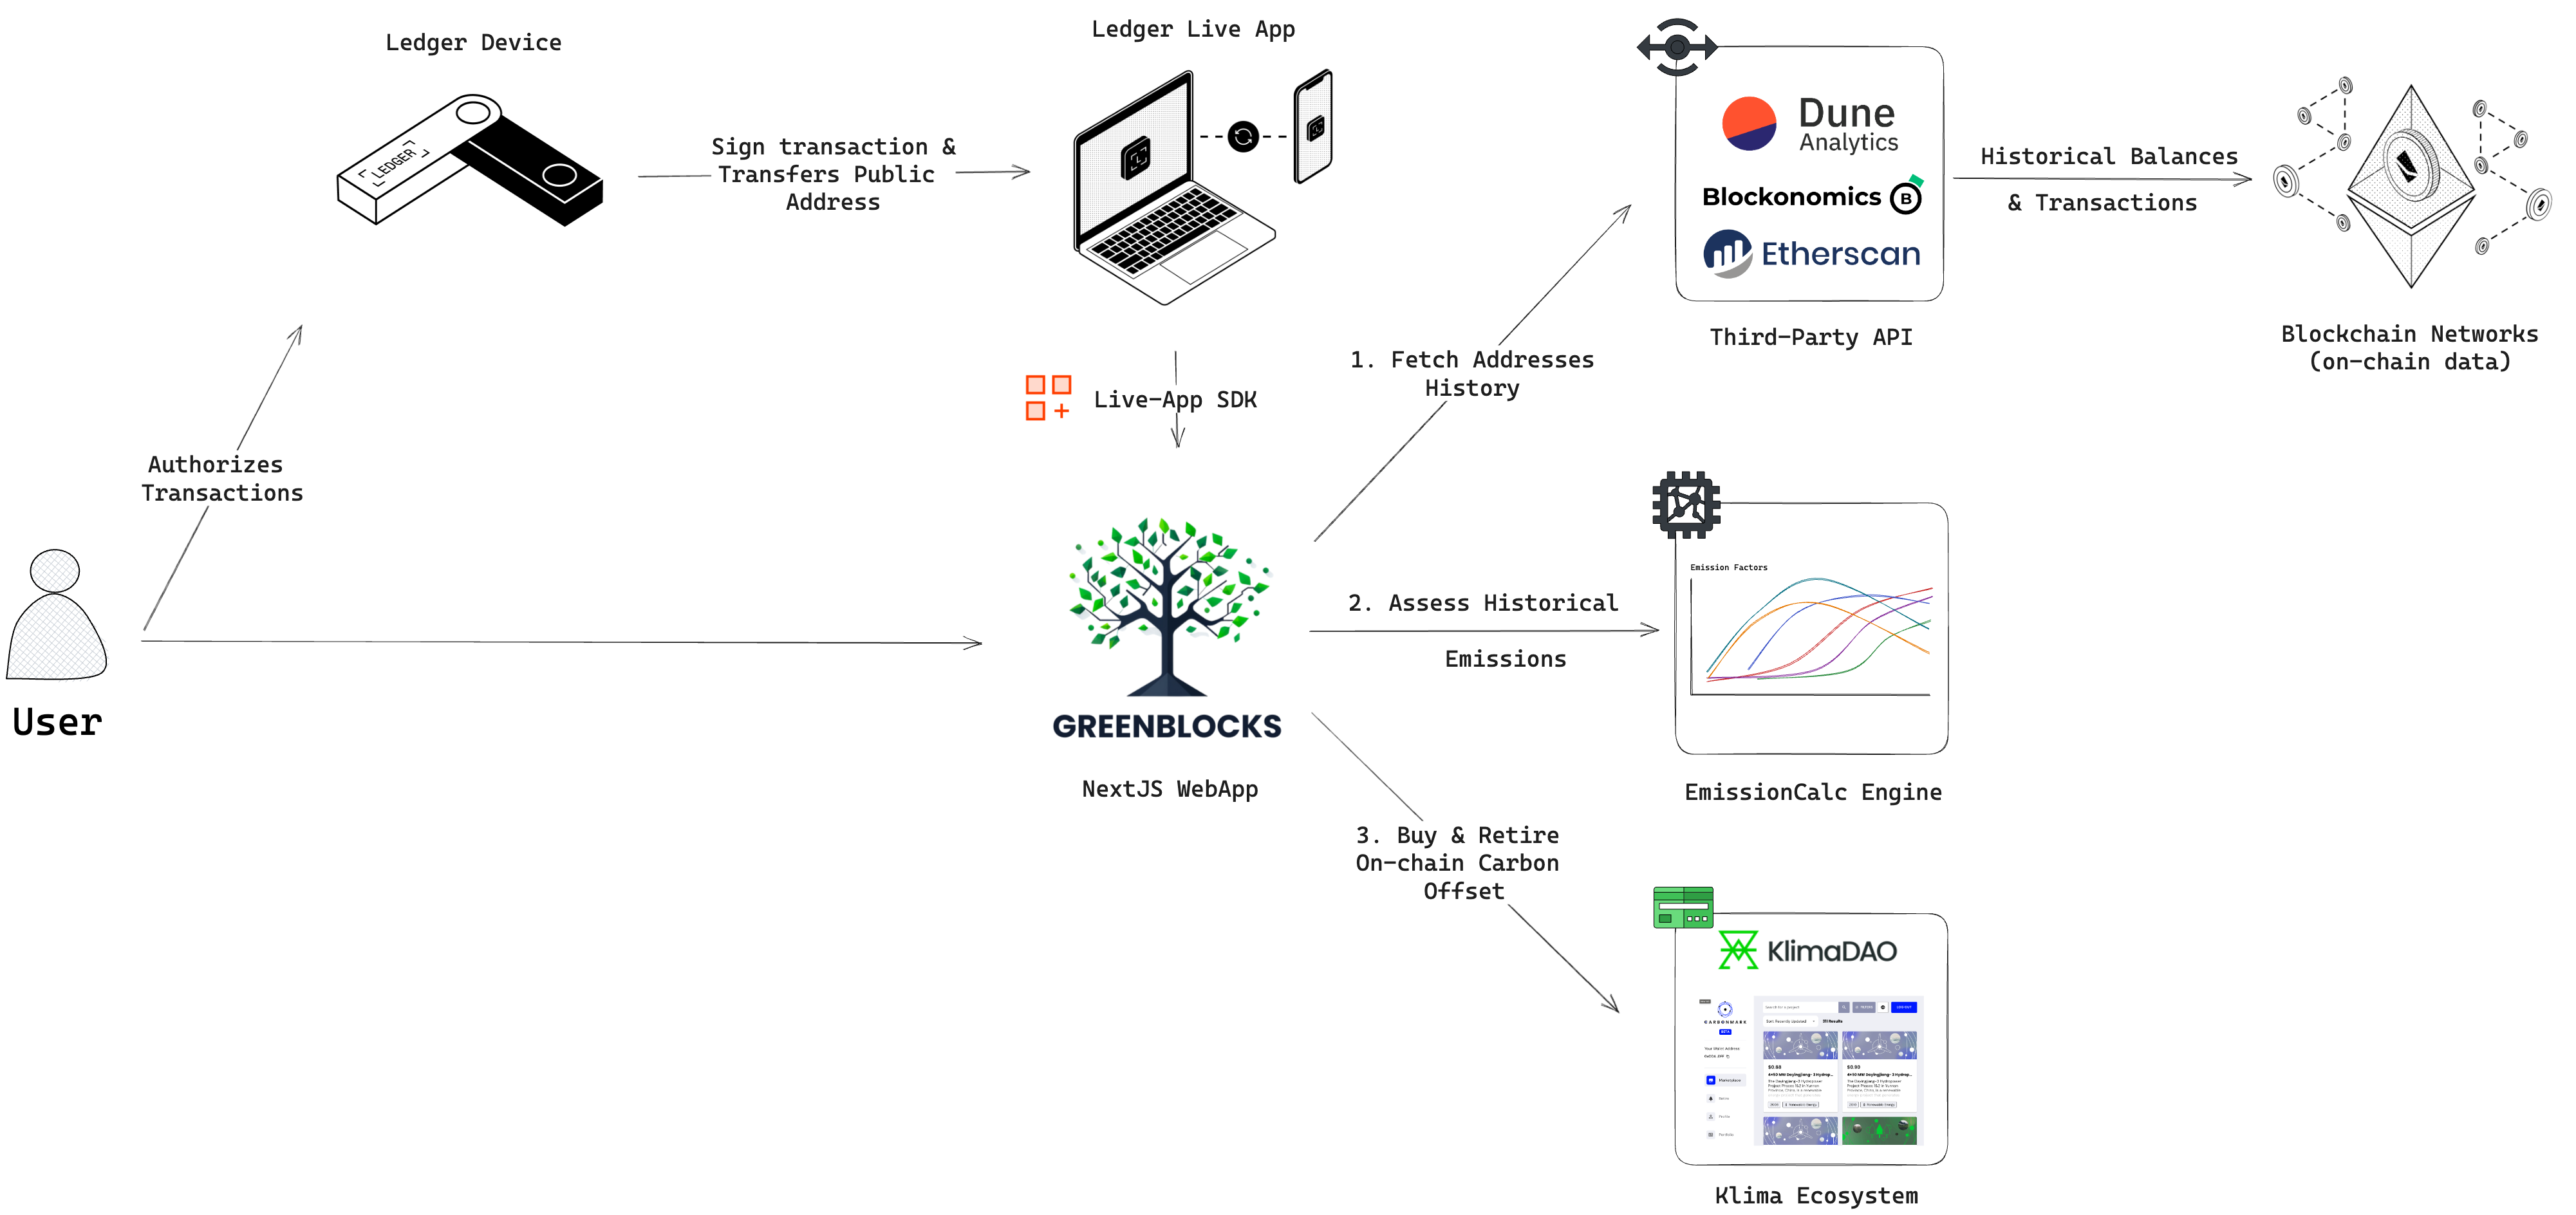
\includegraphics[scale=0.125]{figures/greenblocks_functionnal.png}}
    \caption{GreenBlocks Platform - Functionnal Architecture} 
    \label{fig:functionnal_architecture}
\end{figure}
\change{Review figure width}
\blindtext
\subsection{System Architecture and Components}
\subsection{User Interface Layer}
\subsection{Middleware Layer}
\subsection{Backend Layer}
\subsection{Data Layer}
\subsection{Development Process}
\section{Discussion}
\subsection{Comparative Analysis: Different User Profiles}
\subsection{Limitations and Future Work}

\section{Conclusion}

\section{References}
\bibliography{bibliography.bib}


\end{document}